%-----------------------
% Title page
%-----------------------
\begin{titlepage}
  \centering

  \textsc{ELEC4630 Assignment 1}\\
  \vspace{9cm}

  \rule{\linewidth}{0.5pt}\\

  \vspace{1em}
  \LARGE\textsc{Question 3}\\
  \vspace{1em}

  \LARGE\uppercase{\textbf{{Hough Transforms}}}\\

  \rule{\linewidth}{2pt}\\

  \vfill

  \normalsize{Deren Teo (4528554)}
  \vspace{1cm}

\end{titlepage}

%-----------------------
% Report body
%-----------------------
\section{Introduction}

The Hough transform is a technique that can be used to detect any shape in an image, as long as the shape can be represented in mathematical form \cite{opencv_hlt}. This report presents a method of using the Hough line and circle transforms to identify various features in an image of Mr Bean and his car. The features of interest are the edge of the road, Mr Bean's broomstick and the wheel hubs of Mr Bean's car.

\section{Background Theory}

\subsection{Hough Line Transform}

\textit{(Please refer to Question 2 response.)}

\subsection{Hough Circle Transform}

The Hough circle transform (HCT) is similar to the Hough line transform (HLT), though there are a few key differences \cite{opencv_hct}. The HCT operates in Cartesian coordinates, in which a circle is defined by the parameters $x$, $y$ and $r$:
\begin{align}
  (x - a)^2 + (y - b)^2 = r^2
\end{align}

The HCT defines an accumulator, and for each white pixel, iterates over every parameter combination defining a unique circle to search the image for circles of varying size \cite{korting_hct}. When the algorithm finishes, circles appear in the Hough space as parameter combinations with more than a thresholded value of associated pixels \cite{korting_hct}. However, because the equation of a circle has three parameters, the accumulator is a three-dimensional tensor \cite{wikipedia_hct}. As a result, the algorithm is significantly more computationally expensive compared to the HLT.

For this reason, often a reduced implementation of the HCT is implemented, where a known radius is required, such as for MATLAB's \texttt{imfindcircles} function \cite{mathworks_imfindcircles}. This reduces the size of the search space, but also makes the algorithm less powerful when the radius is unknown or circles of multiple radii are present in the image.

An alternative is the Hough gradient method, which first involves using edge detection to identify possible circle centres, then finds the best radius for each candidate centre \cite{opencv_hct}. This is the method used by OpenCV's \texttt{HoughCircles} function \cite{opencv_hct}. While this method retains the ability to detect circles of all sizes, for efficiency reasons the implementation is more complex than the standard Hough transform \cite{opencv_hct}, and is therefore more difficult to intuitively tune.

\subsection{Morphological Transformations}

Morphological transformations are a set of operations performed on a binary image which alter the shape of the image details \cite{opencv_mt}. They operate on the convention that the image foreground is white and the background is black \cite{opencv_mt}. Five morphological transformations are relevant to the solution presented in this report.

\subsubsection*{Erosion}

Erosion ``erodes'' the foreground around the edges by convolving the image with a kernel \cite{opencv_mt}. A pixel in the original image is only retained if all pixels under the kernel are white \cite{opencv_mt}. Erosion may be useful for removing noise, or disconnecting thinly-connected areas in the foreground \cite{opencv_mt}.

\subsubsection*{Dilation}

Dilation is the opposite of erosion; pixels are added around the foreground edges by the convolution \cite{opencv_mt}. A pixel is white if any pixels under the kernel are white \cite{opencv_mt}. Dilation is useful for joining broken sections of the foreground, and is commonly used with erosion to remove noise while maintaining the foreground geometry \cite{opencv_mt}.

\subsubsection*{Opening}

Opening refers to erosion immediately followed by dilation using the same kernel \cite{opencv_mt}. As mentioned, this is often useful for removing noise \cite{opencv_mt}.

\subsubsection*{Closing}

Closing is the opposite of opening; dilation followed by erosion \cite{opencv_mt}. This is often useful for closing small holes in foreground objects \cite{opencv_mt}.

\subsubsection*{Top Hat}

The top hat operation produces the difference between an image and its opening \cite{opencv_mt}. The outcome is similar to removing areas within the foreground in which the kernel entirely fits, resulting in large foreground areas being removed, leaving only the finer details.

\subsection{Canny Edge Detection}

The Canny Edge detector is a popular edge detection algorithm for its low error rate, good localization and minimal response (only one detector response per edge) \cite{opencv_canny}. The Canny Edge detection process follows the following four steps \cite{opencv_canny}:
\begin{enumerate}
  \item Noise is filtered out using a Gaussian filter.

  \item The intensity gradient of the image is determined by applying a pair of convolution masks (in the $x$ and $y$ directions), then calculating the gradient vector.

  \item Non-maximum supression is applied to remove pixels that are not part of an edge, leaving only candidate edges.

  \item Using two thresholds (provided as algorithm parameters), pixels forming candidate edges are filtered by their gradient. If the gradient is higher than the upper threshold, the pixel is accepted as part of an edge. If the gradient is lower than the lower threshold, the pixel is rejected. If the gradient is between the thresholds, it is only accepted if it is connected to a pixel above the upper threshold.

\end{enumerate}

The ratio of upper to lower thresholds is generally recommended to be between 2:1 and 3:1 \cite{opencv_canny}.

\subsection{Contours}

A contour is a curve defined around the border of a number of connected points with the same colour or intensity \cite{opencv_contour}. In image processing, contours are useful for shape detection and recognition \cite{opencv_contour}. A fast and effective method for contour detection is presented by Suzuki and Abe \cite{suzuki_1985}, and is the method used by the OpenCV \texttt{Canny} function \cite{opencv_bib}.

The precise mechanics of the Suzuki and Abe \cite{suzuki_1985} algorithm are well beyond the scope of this report. However, as a very brief overview, both variants of the algorithm leverage graph properties of a binary image to create an image representation and extract features without reconstructing the image \cite{suzuki_1985}. The difference between the variants lies in whether the algorithm follows only the outermost borders, or also hole borders \cite{suzuki_1985}.

\newpage
\section{Methodology}

The presented solution is composed of three distinct sub-solutions, one for each of the desired features. The solutions are executed in sequence to produce the desired result.

First, for detecting the road edge:
\begin{enumerate}
  \item The image is converted to HSV and the saturation channel is extracted, which contrasts the road well against the grass.

  \item The image is binarized using an experimentally tuned threshold of 100. This separates the road from the rest of the background.

  \item The binarized image is morphologically closed using a very large kernel (121 x 121) to remove all detail except for the road edge border, which is possible because the road edge is the largest and most clearly defined detail in the binarized image.

  \item Canny Edge detection is performed to define the road edge for the Hough line transform.

  \item The Hough line transform is then applied with an experimentally tuned threshold of 125 to identify the road edge. This threshold effectively filters out all noise.

  \item Using the method described in the Question 2 methodology, an equation for the road edge line is defined. The start and end points of each section of the road edge are not yet determined.

  \item To determine the start and end points of each road section, contour detection is performed on the morphologically closed image. This finds the position and size of each road section.

  \item Finally, the position and size of each road section are used to determine the start and end points of the road edge.

\end{enumerate}

Then, for detecting Mr Bean's broomstick:
\begin{enumerate}
  \item The image is converted to HSV and the saturation channel is extracted, which contrasts the broomstick fairly well against the grass.

  \item The image is binarized using an experimentally tuned threshold of 150. This separates the broomstick from most of the background but produces a noisy image.

  \item The morphological top hat transform is applied using a vertical kernel to black out large white sections without erasing the broomstick. This primarily removes Mr Bean and the car, leaving the broomstick as the largest remaining foreground shape.

  \item The image is morphologically opened to remove some of the noise before applying the Hough line transform. A vertical kernel is again necessary to avoid erasing the broomstick.

  \item The Hough line transform is applied with a threshold tuned to ignore the remaining noise. After the morphological transforms, the broomstick should be the only detected line.

  \item Using the method described in the Question 2 methodology, the equation for the broomstick line is derived. However, the extents of the line are not yet known.

  \item To detect the extents of the line, contour detection is performed and the contours are sorted by height. The position and size of the largest contour are assumed to represent the broomstick.

  \item Using the position and size of the broomstick contour, the extents of the broomstick line can be determined.

\end{enumerate}

\newpage

And finally, for detecting the wheel hubs of the car:
\begin{enumerate}
  \item The image is converted to grayscale and binarized using an experimentally tuned threshold of 50. This contrasts the wheel hubs strongly against the tires.

  \item The image is morphologically closed to remove noise, then contour detection is performed to identify circular contours.

  \item The contours are filtered by area to leave only wheel-sized contours. The wheels in the image are approximately 3000 sq. pixels, and the contours are filtered to between 2500 and 3500 sq. pixels.

  \item The contours are further filtered by aspect ratio, which is sufficient to distinguish the wheel hubs. The aspect ratios between 0.8 and 1.2 are kept.

  \item A bounding rectangle is used to find the size and shape of the remaining contours, which can define circles of respective positions and radii. Where the aspect ratio is not 1, the circle diameter is taken as the average of the bounding rectangle width and height.

\end{enumerate}

\section{Results}

Figure \ref{fig:q3results} presents the image with red lines demarcating the identified features: the edge of the road, Mr Bean's broomstick, and the wheel hubs of Mr Bean's car.

\begin{figure}[ht]
  \centering
  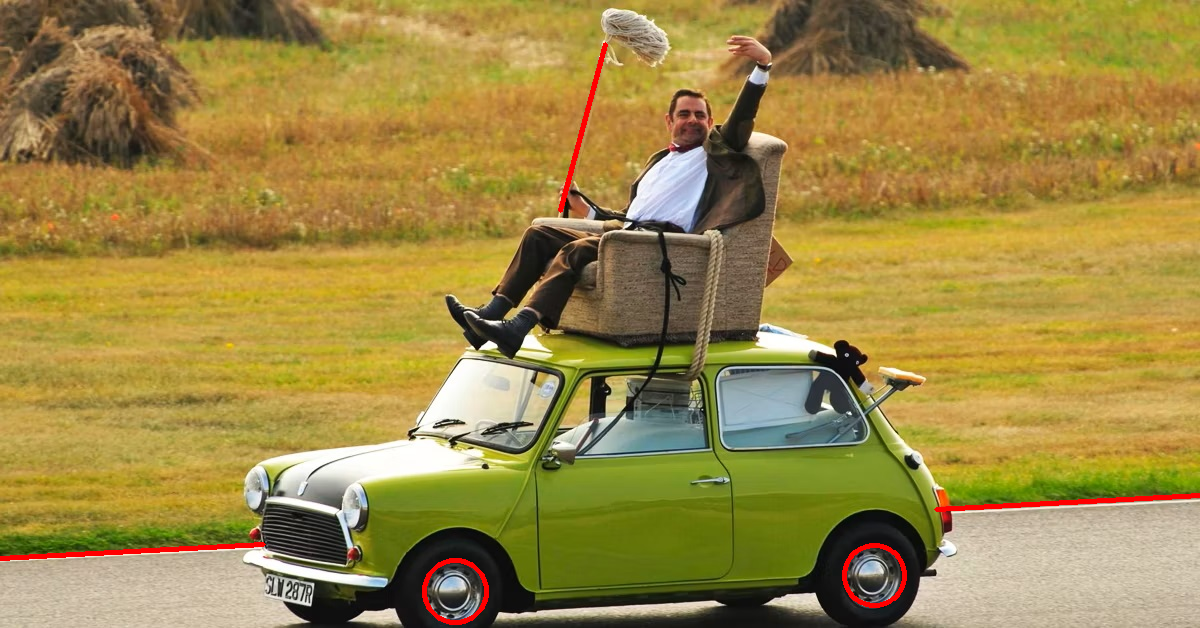
\includegraphics[width=0.6\textwidth]{images/q3_results.png}
  \caption{Features detected using contour detection and Hough transforms.}
  \label{fig:q3results}
\end{figure}

\newpage
\section{Discussion}

This report has presented a method of detecting several features in an image of Mr Bean and his car. The features of interest are: the road edge, Mr Bean's broomstick and the wheel hubs of Mr Bean's car. The method succesfully identifies all features, evident in Figure \ref{fig:q3results}.

There are, however, certain caveats to the solution which warrant further discussion.

Firstly, in detecting the road edge, the binarized image is morphologically closed using a very large kernel to remove all details except the road edge. This assumes the road edge is the most significant feature in the image, and will therefore remain after all other details are erased. If this is not true, for example if the car is near either side of the frame, the edge may not be properly detected. Furthermore, contour detection is used to identify the road sections in the closed image, which allows any number of road sections to be detected, anywhere in the image. However, it also assumes the only features remaining in the closed image are sections of the road. If this is untrue, road edges will be incorrectly identified.

Secondly, in detecting the broomstick, a manual vertical offset is implemented to account for the solution slightly misidentifying the position of the broomstick. The Hough line transform successfully identifies the broomstick line; however, when performing contour detection to identify the broomstick extent, the solution includes part of the chair and excludes the top of the broomstick. This is due to the extensive morphological operations performed to reduce noise disturbing the broomstick endpoints.

Finally, in detecting the wheel hubs, the Hough circle transform is not used. In spite of the aim of the question, it was found that pure contour detection provided a faster, simpler and more robust method of wheel detection than the Hough circle transform. The predominant reason is that the Hough circle transform requires the size of the wheels to be known. This necessitates a contour detection to identify circular shapes and provide their sizes. Yet, having already identified the circular shapes, there is no further need to apply the Hough circle transform.

\section{Conclusion}

In summary, this report presents a successful solution to the problem of identifying several features in an image of Mr Bean. The solution successfully identifies visible sections of road edge, Mr Bean's broomstick, and the wheel hubs of Mr Bean's car. However, shortcomings with the solution are present and discussed, largely surrounding the unknown level of robustness required of the solution.
